% set document class
\documentclass[a4paper,notitlepage,12pt]{article}

% load packages
\usepackage[utf8]{inputenc}
\usepackage[a4paper, margin=0.8in]{geometry}
\usepackage{authblk}
\usepackage[english]{babel}
\usepackage{graphicx}
\usepackage{indentfirst}
\usepackage{xr-hyper} % for cross-referencing between documents
\usepackage{hyperref}
\usepackage{apacite}
\usepackage{float}
\usepackage{amsmath}
\usepackage[flushmargin]{footmisc}
\usepackage[flushleft]{threeparttable}
\usepackage{array}
\usepackage[font=small, labelfont=it]{caption}

% specify footnote margins
\renewcommand\footnotelayout{%
  \advance\leftskip 0.7cm
  \advance\rightskip 0.7cm
 } 

% specify bibliography and link style
\bibliographystyle{apacite}
\hypersetup{
    colorlinks=true,
    linkcolor=blue,
    filecolor=magenta,      
    urlcolor=cyan,
    citecolor=blue
}
\renewcommand\bibliographytypesize{\small}

% specific images path relative to the main .tex file 
\graphicspath{ {./figures/} }

% specify some custom commands
\renewcommand{\baselinestretch}{1.2}
\renewcommand*{\Authsep}{, }
\renewcommand*{\Authand}{, }
\renewcommand*{\Authands}{, }
\renewcommand*{\Affilfont}{\normalsize}

% set up the author block
\setlength{\affilsep}{2em}   % set the space between author and affiliation
\author[1]{Samuel Zorowitz}
\author[1,2]{Daniel Bennett}
\author[1,3]{Yael Niv}
\affil[1]{Princeton Neuroscience Institute, Princeton University, USA}
\affil[2]{Department of Psychiatry, Monash University, Australia}
\affil[3]{Department of Psychology, Princeton University, USA}

% specify the title
\title{Inattentive responding can induce spurious associations between task behaviour and symptom measures}

% turn date off
\date{}

% Define paragraph formatting
\setlength{\parindent}{0em}
\setlength{\parskip}{1em}

\begin{document}

\maketitle

% make abstract
\abstract{Abstract}

% page break before introduction
\clearpage

% Define paragraph formatting
\setlength{\parindent}{0em}
\setlength{\parskip}{1em}

\section{Introduction}

In recent years, online labor markets (e.g. Amazon Mechanical Turk, Prolific, Crowdflower) have become increasingly popular as a source of research participants in the behavioral sciences \cite{stewart2017crowdsourcing}, largely due to the ease with which these services allow for collecting large, diverse samples. Similarly, the advantages of online data collection platforms have been recognized for clinical research \cite{chandler2016conducting} and are increasingly used in studies of computational psychiatry. Here they are offer additional advantages. The ability to collect large samples facilitates transdiagnostic analysis, studying symptom co-occurrence and relation to behaviors \cite{gillan2016taking, rutledge2019machine}. Online platforms makes it easier to recruit and study otherwise difficult-to-reach populations \cite{strickland2019use}. Online platforms also make re-recruitment easier, making it possible to validate the reliability of measurements tools \cite{enkavi2019large} and possibly study longitudinal processes over long timescales \cite{kothe2019retention}. Some examples here: gillan


Paragraph 2: These advantages not without costs: online means giving up the control of the laboratory. Participants may be distracted, multi-tasking, and with different incentives than usual in-lab participants. Fortunately, many previous studies have found data quality on online crowdsourcing websites not altogether different or worse than in-lab samples. This isn't to say bad data doesn't exist: estimates vary, but non-negligible data bad and new issues arise. For the most part, however, noise has been treated as unsystematic something that can be overcome with increased samples  \cite{gillan2016taking, chandler2020participant}. 

> Although typical undergraduate subject populations are often motivated to participate in studies because of an interest in psychology, MTurk participants are unsupervised and anonymous, complete surveys in unknown locations, and are motivated by financial incentives

We specifically want to draw attention to a less appreciated fact: when traits are rare, such as in psychiatry, careless responding is more likely to manifest as symptom endorsement \cite{chandler2020participant, ophir2020turker}. Rather than mask true correlations, this can induce spurious correlations in data. This effect is well documented in personality psychology, where the presence of careless respondents can induce correlations between questionnaires and bias estimated factors in factor analysis. To our knowledge, however, discussion of this point has been limited to associations between self-report measures and not with respect to behavioral experiments. There is no reason to expect, however, that this result should be limited to those domains and may similarly be an issue for computational psychiatry.

Paragraph 4: not enough to speculate -- must demonstrate this is an issue. what we gonna show: (a) the minority of individuals screen. (b) behavior and survey screens may not correlate. (c) these correlations do arise. We close with some recommendations based on simulations. 

\section{Core Problem}

In this first section, we illustrate the core problem: namely, how C/IE responding can give rise to spurious correlations between measures of task behavior and self-reported symptoms. For our example, we have in mind a typical use case in computational psychiatry: a researcher runs a study involving a behavioral task and at least one self-report symptom measure. Specifically, we have in mind tasks where the primary outcome measure is an index of decision making. That is, we are primarily concerned with tasks where on each trial a participant must decide how to respond to some stimuli. This decision may be what is the appropriate response given some rule (e.g. color-naming in the Stroop task), which stimulus is greater (e.g. dot-motion in perceptual decision making, or which stimulus is the most valuable (e.g. decisions from description, bandit tasks). Importantly, what all of these tasks share is an explicit or implicit rule for accuracy. That is, we are not measuring idiosyncratic preferences: attentive participants should respond in a coherent and consistent fashion (e.g. prefer more valuable to less valuable).

To illustrate how C/IE responding can give rise to spurious correlations in these paradigms, we introduce a simple computational framework relating responding on behavioral and self-report measures. Beginning first with task behavior, we assume that a decision, $y_{i,j}$, with $k$ response levels made by participant $i$ on trial $j$ is governed by:

\begin{equation}
    p(y_{i,j} = k \mid \psi_i, \pi_i) = (1-\pi)\text{Cog}(\psi_i) + \frac{\pi}{k}
\end{equation}

Here, $\psi_i$ is the set of latent parameters of a cognitive model governing behavior on a particular task. For example, $\psi_i$ may correspond to the parameters of a drift diffusion model or Q-learning model. More importantly, $\pi_i$ is a lapse rate which controls the degree of C/IE responding. Specifically, a participant always responds consistent with the internal model when $\pi=0$, but only responds randomly when $\pi=1$. We note that this definition assumes that C/IE responding manifests only as statistically random responding. As will be discussed below, we believe this is an overly simplistic assumption, as there exist a great multitude of low-effort heuristic strategies beyond random responding a participant may engage in. We make this assumption in this section strictly for illustrative purposes.

Turning now to self-report behavior, we assume that a response, $y$, with $k$ response levels made by participant $i$ to item $j$ is governed by:

\begin{equation}
    p(y_{i,j} = k \mid \phi_i, \pi_i) = (1-\pi)\text{IRT}(\phi_i) + \frac{\pi}{k}
\end{equation}

Here, $\phi_i$ is a set of latent item response parameters governing a participant's pattern of endorsement (for a review see Burkner). Again, $\pi_i$ is a lapse rate. As above, we assume that C/IE responding manifests as statistically random responding (i.e. equal likelihood of endorsing all response levels). Of course, there exist alternate forms of C/IE responding on self-report measures (e.g. straight-lining, zig-zagging). To reiterate, we make this assumption for strictly illustrative purposes. 

Crucially, we assume that the degree of C/IE responding by modality is related across individuals. That is, we assume a correlation between $\pi$ and $\pi$ such that participants more likely to engage in C/IE responding on one measure is also more likely to engage in C/IE responding on the other. As will be discussed below, we do not assume that the degree of C/IE responding for an individual is identical across modalities (i.e. $\pi \neq \pi$). Participants may be more (or less) motivated to respond carefully on certain modalities for a variety of reasons (e.g. task difficulty, participant abilities, monetary incentives). Regardless, we assume there exists some shared variance in C/IE responding by modality across individuals.  

To illustrate how spurious correlations may arise, we used this framework to simulate four datasets under varying conditions (Figure 1). In each dataset, we simulated 1000 participants responses to both a behavioral and self-report measure. Crucially, we manipulated two key variables: the fraction of C/IE respondents and the skewness of the distribution of self-report scores. Specifically, we manipulated whether the fraction of C/IE respondents was 0\% (Figures 1a, 1c) or 15\% (Figures 1b, 1d), a rate similar to what has been reported in the literature. We independently manipulated whether the skew of the self-report total scores was symmetric (Figures 1a, 1b) or right-skewed (Figures 1c, 1d). We then computed Spearman correlations between behavior and self-report for 1000 random subsamples of 100 participants.

\begin{figure}[!b]
    \centering
    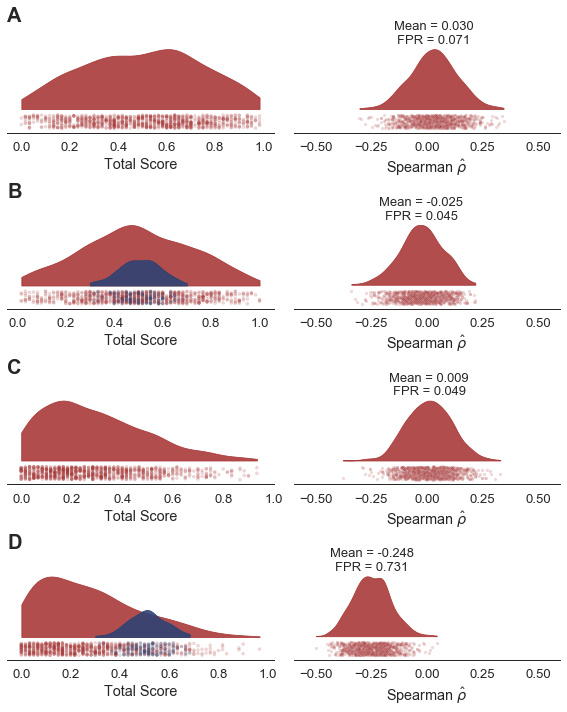
\includegraphics[scale=0.6]{figures/figure_01.png}
    \caption{Caption}
    \label{fig:simulations}
\end{figure}

We draw your attention to two key results of this simulation. First, under a model of statistical randomness, C/IE respondents will fall to the center of the range of total scores. This follows naturally from the definition of statistically random responding (i.e. the mean of a uniform distribution is the center of its range). As such when the distribution of total scores is symmetric, C/IE respondents will resemble the modal participant. However, when the distribution of total scores is asymmetric, C/IE respondents will show elevated (attenuated) total scores when the distribution is right-skewed (left-skewed). That is, for skewed symptom measures where higher scores indicate greater pathology, C/IE respondents will falsely appear as endorsing higher levels of illness.


Most importantly, this has consequences for the experimenter correlating behavior and self-report measures. In the absence of C/IE respondents, regardless of total score distribution, behavior-symptom correlations are centered at zero with false positive rates around the 5\% level (Figures 1a, 1c). Similarly, the presence of C/IE respondents does not impact behavior-symptom correlations when the total score distribution is symmetric (Figure 1b). When the total score distribution is asymmetric, however, the presence of C/IE respondents means the distribution of behavior-symptom correlations is no longer centered at zero and the false positive rate is substantially elevated (Figure 1d). In other words, the combination of asymmetric total scores and C/IE responding yields favorable conditions for spurious behavioral-symptom correlations. Crucially, this is precisely the sort of condition we find ourselves in psychiatry, where many symptoms of interest have low overall endorsement in the general population.

Thus, we have shown how spurious behavior-symptom correlations may arise in presence of C/IE respondents. However, as panel 1c suggests, removing these participants should prevent or decrease the likelihood of spurious correlations. Thus the question next turns to how common is this scenario. 

Before moving on, we wish to address one portion of our assumptions: namely statistically random responding for self-report measures. Random responding in one heuristic pattern, but there are others. For example, C/IE participants also show straight-lining (i.e. choosing the same response level for most or all items) and zig-zagging (i.e. choosing adjacent response levels of successive items). We note that these heuristic strategies will also give rise to these problems in aggregate. By definition, zig-zagging will yield approximately uniform response patterns. In aggregate, a collection of straight-liners choosing different response levels will form a uniform distribution in aggregate that will also yield similar patterns of correlations.

[supplementary figure?]

\section{State of screening practices}

As demonstrated in the preceding section, the presence of C/IE respondents can yield spurious correlations between measures of task and self-report behaviors in scenarios common to psychiatry. As such, it is imperative for researchers to detect and remove these participants prior to analysis. This raises two questions: (1) do researchers screen participants of online studies for C/IE responding, and if so (2) what how do they do so? The answers to these questions should, in part, tell us how worried we need to be about the above pattern of results.

In this section, we conduct a cursory review of the literature to evaluate the state of screening practices in online studies of psychiatric behavior. Studies were identified through a set of searches in Google Scholar entailing permutations of keywords related to online labor platforms (e.g. "online", "mechanical turk", "prolific"), psychiatry, and behavioral tasks. Studies were included in the review insofar that they met the following criteria: (a) recruited participants online, (b) collected responses on at least one self-report symptom measure, and (c) collected responses to at least one experimental task. Using these criteria, we identified 49 studies suitable for inclusion (the complete list of studies and their associated search queries are included in the supplement). Next, we reviewed the methods of each study to identify whether (a) participants were excluded (or adjusted for) based on task and/or self-report behaviors and if so (b) what criteria were used. We note that the goal of this review was not to be exhaustive, but rather to provide a representative overview of the practices common in this subfield.

Summary statistics about the prevalence and types of screening are provided in Table 1. Turning first to exclusion criteria based on task behavior, the majority of studies in our sample (39/48; 81\%) used at least approach to identify C/IE respondents in task behavior. Of those studies, just over half used only one form of evaluation. Unsurprisingly, there was considerable heterogeneity in the methods used to screen task behavior across studies. Most common was screening based on performance accuracy (numbers), or responding above chance levels. Almost as common was screening based on response variability (numbers), or using. Less common methods were screening based on response times and failed comprehension checks. Briefly, we note that many studies excluded based on missing data but we do not consider that here as that many not reflect C/IE responding, but instead technical issues. In sum, the majority of studies utilized at least one method for screening behavioral data (though the method(s) used varied considerably across studies). 

By comparison, only the minority of studies performed at least one form of screening for C/IE responding in self-report data. The majority of studies performing self-report screening employed only one method. By far, the most common method was the use of attention checks. Attention checks can be subdivided into different categories. For example, instructed items explicitly tell a participant which response option to choose; those failing to do so are presumably C/IE respondents. In contrast, infrequency items are those which have only one or a small set of valid responses. Most attention checks fell into the former category; only one study in sample reported using infrequency items. Most other studies using attention checks did not disclose the check they used; though there are valid reasons for doing so, this prevents us from knowing their methods. Far less were so-called unobtrusive or statistical methods. Only a handful of studies reported using screening based on personal consistency with repeat items, entropy, or outlier detection. 

To summarize whereas screening for C/IE responding in task behavior is ostensibly the norm, screening self-report behavior is far less prevalent. Indeed, whereas approximately 80\% of studies used at least one method for screening behavioral data, fewer than 40\% of studies did the same for self-report data. One possible explanation for this pattern of results is that researchers assume that screening methods for task and self-report behaviors are equally sensitive to C/IE responding. That is, researchers may believe that both types of screening measures will detect the same participants and are as such redundant. If this is the case, to our knowledge this assumption has yet to be empirically demonstrated. Thus, we ran an experiment blah blah blah.

Before moving on, we pause to discuss two important pattern of results from this literature review. First, we found that the majority of studies used only one single method to detect C/IE responding. This is concerning for several reasons. First, multiple empirical investigations of self-report screening metrics have demonstrated that different metrics are sensitive to different heuristric strategies and employing only one may mean missing other bad data. Though this has been less researched in the. context of task behavior, it is likely no less true. For example, WSLS and accuracy. Similarly, metrics are a SNR issue and multiple metrics allow for better resolution of true and false positives. 

Second, and more controversially, that the majroity of studies using instructed items is ocncerning. Less effective on MTurk. Empirical evidence that folks know to look for them. Popularly discussed on formums (link 1, linke 2). In our studies, have found less sensitive measure than others. We encourage researchers to swap or at least use multiple.  


\begin{tabular}{ |p{3cm}||p{3cm}|p{3cm}|p{3cm}|  }
 \hline
 \multicolumn{2}{|c|}{Behavioral Screening} &
 \multicolumn{2}{|c|}{Self-Report Screening} \\
 \hline
 Accuracy & 18 (37\%) & Attention Check & 17 (35\%) \\
 Variability & 15 (31\%) & Instructed & 10 (20\%) \\
 Response Time & 7 (14\%) & Unspecified &  5 (10\%) \\
 Comprehension & 5 (10\%) & Unobtrusive &  4 (8\%) \\
 Other & 16 (33\%) & &  \\
 \hline
 At least 1 & 39 (80\%) & At least 1 & 19 (39\%) \\
 \hline
\end{tabular}


\section{Methods}

\subsection{Participants}

405 participants were recruited online to participate in a behavioral experiment in May, 2020. Approximately half of participants were recruited from Amazon Mechanical Turk (N=204), whereas the remaining half were recruited from Prolific (N=200). All participants consented to participate. Participants demographics are reported in Table S1. Importantly N participants admitted to participating twice: once on MTurk and once on Prolific, and were removed from all subsequent analyses.  All participants were paid at a rate of \$12/hr plus a performance bonus of up to blah (average rate: blah). All things approved by Princeton. 

400 participants agreed to participate online during month of May 2020. 200 participants from MTurk. 200 participants from Prolific. All participants consented to participate. All participants were paid at a rate of \$12/hr plus a performance bonus of up to blah (average rate: blah). All things approved by Princeton IRB.  

Importantly, participants from MTurk were recruited via CloudResearch (formally TurkPrime). Describe methods. Similarly describe methods for Prolific. Address MTurk screening requirement. 

\subsection{Symptom Measures}

After consenting but prior to start of experiment, participants completed four measures: (1) GAD-7, (2) 7U7D, (3) BIS-BAS, (4) SHAPS. Importantly, these four were selected due to modal responding (two right-skewed, one symmetric, one left-skewed). 

\textbf{GAD-7}

\textbf{7u7d}

\textbf{BIS/BAS}

\textbf{SHAPS}

Describe infrequency items. Describe recommendations, describe cat and mouse situation. Provide one example. All previously vetted. 

\subsection{Reversal Learning Task}

Participants completed a 3-arm probabilistic learning task, similar to [citations]. On every trial, participants were able to choose one of three options. On any trial, there was always one best option, rewarding with 80\% probability; remaining arms rewarded with 20\% probability. Crucially, every 15 trials the contingencies switched such that one of the two suboptimal arms became optimal. Participants completed 90 total trials. Decision phase 2000ms, outcome phase 1000ms. The total experiment lasted 8 minutes.

The cover story was fishing. Three beaches, trying to catch the most fish. Participants explicitly told some beaches better than others, and that the best beach may change over time. Participants had to answer four comprehension check questions: [list questions]. Participants had to complete all comprehension checks to continue, but were never excluded (similar to Gillan). Note that this may have caused attrition.

\subsection{Survey Analysis}

\textbf{Infrequency fail}

\textbf{Entropy}

\textbf{Reliability}

\textbf{Mahalanobis D}

\textbf{Reading Times}

\subsection{Behavior Analysis}

\section{Results}

\subsection{Description}

What participant metadata to include? Percentage of overlap between MTurk and Prolific? 

Description of infrequency item fails. Probably want to describe more fails on MTurk than Prolific. 

\subsection{Agreement of screening metrics}

Paragraph 1: First we compare metrics based on Spearman correlation. 

Paragraph 2: Second we compare metrics based on dice coefficient.

Paragraph 3: In sum, it seems to be that behavior and survey metrics may not always agree. That is, screening on behavior alone is not guaranteed inattentive survey responders. What are the consequences? 

\subsection{Correlation Analysis}

\section{Simulation Results / Recommendations}

\section{Discussion}

Topic XX: Continuum of human effort

Topic XX: not a problem specific to online studies, but probably worse there due to lack of monitoring and different incentives.

Topic XX: how many to expect across platforms and by method. mturk vs. prolific differences. cat and mouse problems.

Topic XX: incentives for performance in online tasks

Topic XX: Accidentally screening out participants of interest

\section{Supplement}

\bibliography{main}

\end{document}
